\documentclass{beamer}
\usepackage{amsmath}
\usepackage{tabularx}
\usepackage{graphicx}
\usepackage{siunitx}
\usepackage{fancyvrb}
\usepackage{times}
\usepackage{booktabs}
\usepackage[normalem]{ulem}
\usepackage[T1]{fontenc}
\usetheme{Warsaw}
\usecolortheme{crane}

\usepackage{listings}
\usepackage{color}


\definecolor{dkgreen}{rgb}{0,0.6,0}
\definecolor{gray}{rgb}{0.5,0.5,0.5}
\definecolor{mauve}{rgb}{0.58,0,0.82}

\lstset{frame=tb,
  language=R,
  aboveskip=3mm,
  belowskip=3mm,
  showstringspaces=false,
  columns=flexible,
  basicstyle={\footnotesize\ttfamily},
  numbers=none,
  numberstyle=\tiny\color{gray},
  keywordstyle=\color{blue},
  commentstyle=\color{dkgreen},
  stringstyle=\color{mauve},
  breaklines=true,
  breakatwhitespace=true,
  tabsize=3
}


\begin{document}
\begin{frame}
\title{\textbf{Simulating calcium handling and buffering at nerve terminals with CellBlender/MCell}}
\author{Jaron Lee}
\maketitle
\end{frame}

\section{Introduction}
\frame
{
    \frametitle{Motivation of this project}
    \begin{itemize}
        \item Modelling in biology is important - widespread applications
        \item Modelling in biology is difficult - requires skills and knowledge which fall outside biology itself
    \end{itemize}
}

\frame
{
    \frametitle{Goals of this project}
    \begin{itemize}
        \item Develop a thorough understanding of the software, biology
        \item Implement a working visualisation of calcium action at nerve terminals 
        \item Parameterise the model to mimic biological conditions where possible 
        \item Document the process to allow for easy replication 
    \end{itemize}
}
\frame
{
    \frametitle{Software}
    \begin{itemize}
        \item MCell - background Monte-Carlo simulation command-line tool
        \item Blender - 3D animation and design software
        \item CellBlender - interface between Blender and MCell
        \item Python - general-purpose programming language
    \end{itemize}
}


\frame
{
    \frametitle{Advantages of the approach}
    \begin{itemize}
        \item The method developed essentially eliminates the need for the user to be proficient in programming 
        \item Simulation results are presented in animation form - easy to interpret
        \item Easy to adapt the model to answer different scientific questions
    \end{itemize}
}
\section{Background Information}

\frame
{
    \frametitle{An overview of synaptic transmission}
    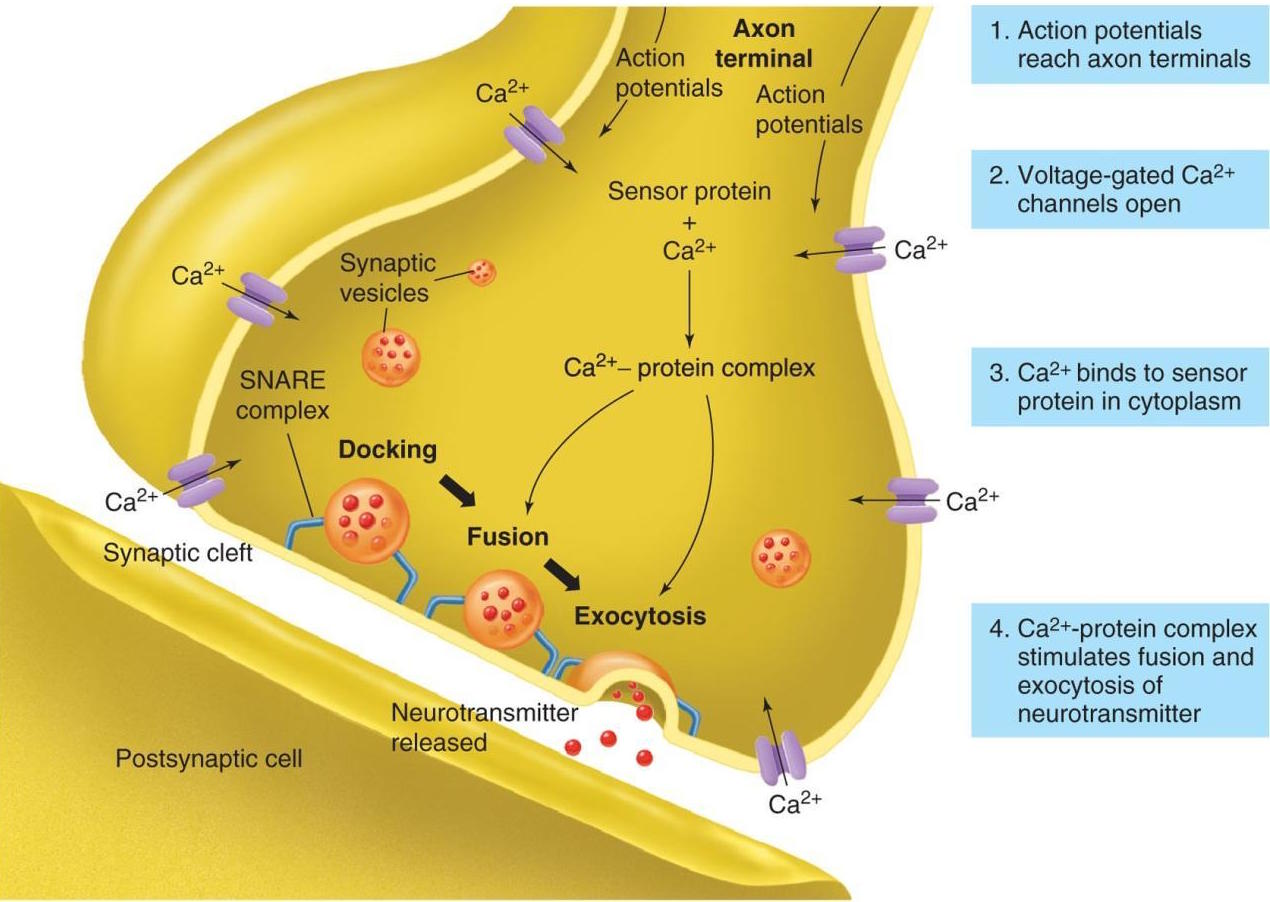
\includegraphics[width=1\textwidth]{fig1.jpg}
}


\section{The Modelling Approach}
\frame
{
    \frametitle{Summary}
    Two phases - presynaptic and postsynaptic
    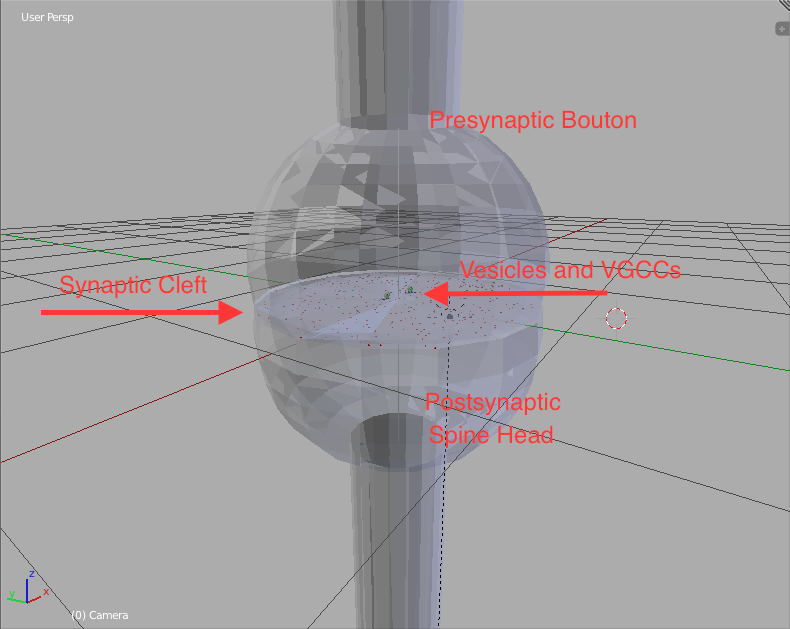
\includegraphics[width=1\textwidth]{fig2.png}
}

\frame
{
    \frametitle{Presynaptic}
    \begin{itemize}
        \item Simulate calcium ion movement
        \item Simulate calcium binding to SNARE complex (Need two calcium to activate)
        \item Record time of vesicle fusion (require three activated SNARE complexes on a vesicle)
    \end{itemize}
}

\frame
{ \frametitle{A question}
    \begin{itemize}
        \item Why not do everything in one step?
        \item The activation of SNARE complexes is randomly determined during the simulation (depends on the movement of calcium ions)
        \item The release of neurotransmitter must be specified before the simulation is run (due to the way CellBlender defines molecule placement and release)
    \end{itemize}
}

\begin{frame}{Model Components}
\begin{columns}
    \begin{column}{0.47\textwidth}
\begin{enumerate} 
    \item Presynaptic bouton 
    \item Spine head
    \item Voltage-gated calcium channels (2)
    \item Vesicles (2)
    \item Glial cells
\end{enumerate}
    \end{column}
    \begin{column}{0.5\textwidth}
    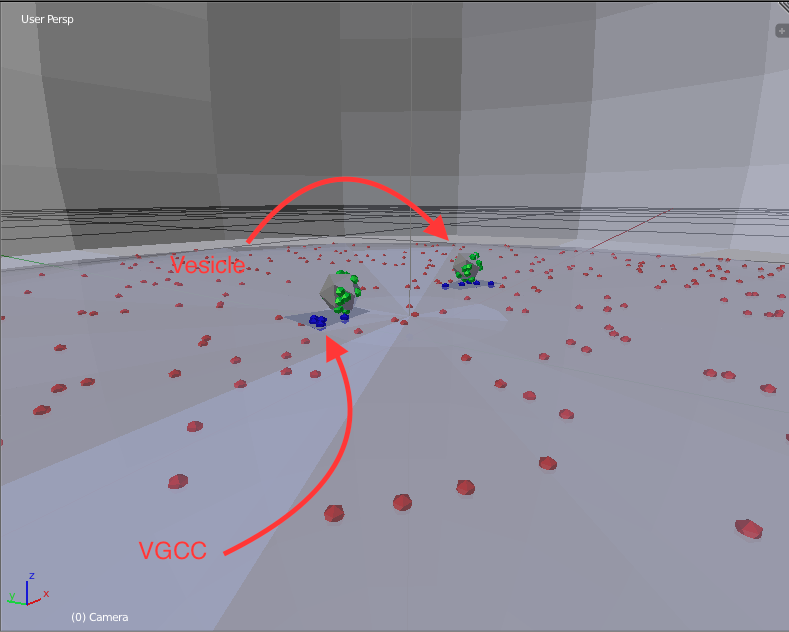
\includegraphics[width=1\textwidth]{fig3.png}
    \end{column}
\end{columns}
\end{frame}

\frame{
    \frametitle{Model Molecules}
\begin{enumerate}
    \item VGCC - the calcium channels responsible for permitting flow of calcium into bouton. Has open and closed states.
    \item Ca - calcium ion
    \item CaBS - a SNARE complex which has a single calcium ion bound
    \item TAG - a SNARE complex which has two calcium ions bound
    \item NT - a neurotransmitter molecule (represents glutamate)
    \item LGIC - a neurotransmitter receptor residing on spine head (receptive to NT). Has open and closed states.
\end{enumerate}
}

\frame
{
    \frametitle{Model Equations}
\begin{table}[H]
\begin{tabular}{ll}
Equation & Description \\ \hline
VGCC\_C $\to$ VGCC\_O & Calcium channel opening \\
VGCC\_O $\to$ VGCC\_C & Calcium channel closing \\
VGCC\_O $\to$ VGCC\_O + Ca & Calcium influx into bouton \\
Ca + CaBS $\to$ CaBS\_Ca & First calcium binding \\ 
CaBS\_Ca + Ca $\to$ TAG & Second calcium binding \\
NT + LGIC\_C $\to$ LGIC\_O& Neurotransmitter binding \\
\end{tabular} 
\end{table}

}

\section{Making the Model Realistic}
\frame
{
    \frametitle{Model Parameters}
    \begin{itemize}
        \item Dimensions
        \item Quantities
        \item Rates
    \end{itemize}
}

\frame
{
\frametitle{Model Rates}
\begin{table}[H]
\tiny
\begin{tabular}{ll}
Parameter & Value \\ \hline
Rate of calcium influx   &  $\SI{1e3}{\per\mole\litre\per\second}$      \\
SNARE complex binding rate & $\SI{1e8}{\per\mol\litre\per\second}$ \\
Glutamate binding rate & $\SI{4.6e6}{\per\mol\litre\per\second}$ \\
Rate of glutamate diffusion & $\SI{4e-6}{\centi\metre\squared\per\second} $      \\
Rate of calcium diffusion & $\SI{5.3e-6}{\centi\metre\squared\per\second} $      \\
Vesicle unzip time & \SI{200}{\micro\second}  \\
Estimate for bouton volume&  $\SI{0.36}{\micro\meter\cubed}$\\ 
Derived estimate for bouton radius & \SI{0.7}{\micro\meter} \\
Estimate for synaptic vesicle radius & $\SI{0.017}{\micro\meter}$ \\ 
Synaptic cleft width &$\SI{0.023}{\micro\meter}$\\
Number of Neurotransmitter molecules per vesicle & 4700\\
Number of Neurotransimtter receptors per spine head & 100 \\
Number of SNARE complexes per vesicle & 15 \\ 
Number of calcium ions to activate synaptotagmin/SNARE & 2 \\
Number of SNAREs to induce vesicle fusion & 3 \\  
Number of vesicles & 750 \\
\end{tabular}
\end{table}
}

\frame{
    \frametitle{Final Result}
    See video...
}
\frame{
    \frametitle{References}
    \begin{itemize}
        \item Synaptic terminal, obtained from https://classconnection.s3.amazonaws.com/811/flashcards/141811/jpg/synapse21329503162446.jpg
    \end{itemize}
}

\bibliography{report_doc}{}

\end{document}
